\section{Neurona biológica}
\subsection{La neurona}

La neurona es un tipo de célula perteneciente al sistema nervioso central, que se comunica tanto por señales eléctricas como por señales químicas. Cada neurona tiene \parencite{sistemaNervioso}:%pag34


 \begin{itemize}
	\item Un cuerpo celular llamado \textbf{soma} que contiene un núcleo y otros componentes celulares.
	\item Una zona de recepción con protuberancias elongadas llamadas \textbf{dendritas}.
	\item Una zona de emisión llamado \textbf{axón}, el cual está compuesto de:
		\begin {itemize}
			\item Cono axónico.
			\item Membrana plasmática axónica y citoplasma.
			\item Recubrimientos de mielina, interrumpido a intervalos regulares por nodos de Ranvier.
			\item Terminales del axón donde se encuentran los botones sinápticos. 
		\end{itemize}
 \end{itemize}


\begin{figure}[h]
 \centering
 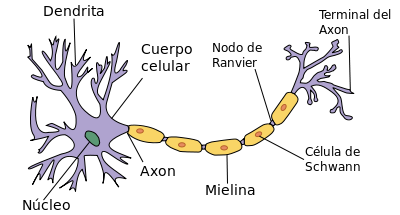
\includegraphics[scale=0.6]{../Figuras/neuronaPartes.png}
 \caption{Neurona, Acracia, 14 January 2007, Wikimedia Commons, \url{https://commons.wikimedia.org/wiki/File:Neurona.svg}, Creative Commons Attribution-ShareAlike 2.5 Generic}
 \label{fig:neuronaP}
\end{figure}

\subsection{Elementos de las neuronas en la transmisión de señales}

Los principales elementos que participan durante la transmisión de señales entre neuronas son:


\begin{itemize}
\item \textbf{Impulsos eléctricos:} potenciales de acción, cambios de voltaje que ocurren a lo largo del axón. % Sucede una vez que se acumularon demasiadas señales a través de las dendritas, entonces la neurona puede disparar un impulso eléctrico, a través del axón, que va a provocar que su terminal libere más químicos, estos químicos son los que hacen los efectos pequeños en cada uno de los cuerpos de las neuronas postsinápticas.
Pueden generar dos efectos en la membrana de la neurona: 
	\begin{itemize}
	\item \textbf{El efecto excitatorio}, despolariza la membrana postsináptica. La neurona es más propensa a mandar un pulso eléctrico.  
	\item \textbf{El efecto inhibitorio}, hiperpolariza la membrana postsináptica. La neurona no manda pulso eléctrico.

	\end{itemize}

\item \textbf{Neurotransmisor/es:} donde se encuentra la sustancia química, %\parencite{sistemaNervioso pag.50.}
son los mensajeros químicos que se comunican entre neuronas adyacentes. La liberación de neurotransmisores de una neurona ayudará a despolarizar o hiperpolarizar (aumentar la magnitud de la carga) de la neurona adyacente, lo que hará que sea más o menos probable que ocurra un potencial de acción en la siguiente neurona.
 
\item \textbf{Plasticidad:} La modificación a largo plazo de las conexiones entre neuronas. %Las neuronas cambian, pirden o forman conexiones que permiten el intercambio de nuevos transmisores sin impulsos eléctricos).
\end{itemize}



En el contexto de la transmisión neuronal de señales, es necesario realizar ciertas distinciones para denotar claramente si una neurona particular está recibiendo o transmitiendo una señal. Las distinciones son las siguientes:
 \begin{itemize}
  \item Neurona presináptica: Transmite una señal a otras neuronas o células a lo largo del sistema nervioso.
  \item Neurona postsináptica: Recibe una señal de otras neuronas o células, procesando y respondiendo a dicha señal.
 \end{itemize}  

La transmisión de señales y almacenamiento de información en las neuronas se da de la siguiente forma:\parencite{neurona_A_cerebro}

\begin{enumerate}
 \item La neurona desde sus dendritas recibe señales de otras neuronas vecinas.
 \item Cada señal se va acumulando en su cuerpo hasta el cono axónico, donde se van a estar sumando la contribución de todos los efectos de cambios de potencial.
 \item En el momento que se rebase un cierto valor umbral, la diferencia de potencial se propaga hasta los botones terminales.
 \item La neurona entra en un período refractario, donde empieza a cambiar el potencial entre el cono axónico y el axón de la neurona.
 \item Se transmite un disparo eléctrico en seguida.
 \item La neurona se va a quedar totalmente quieta, durante un breve momento para que la señal pueda viajar hacia el axón.
 \item Se va a notar un cambio muy violento en el voltaje, que se va recorriendo a lo largo de todo el axón. 
\end{enumerate}

A lo anterior también se le conoce como neurotransmición que esta  descrita con mayor precisión en la figura  \fref{fig:nTransmision}.

\begin{figure}[h]
 \centering
 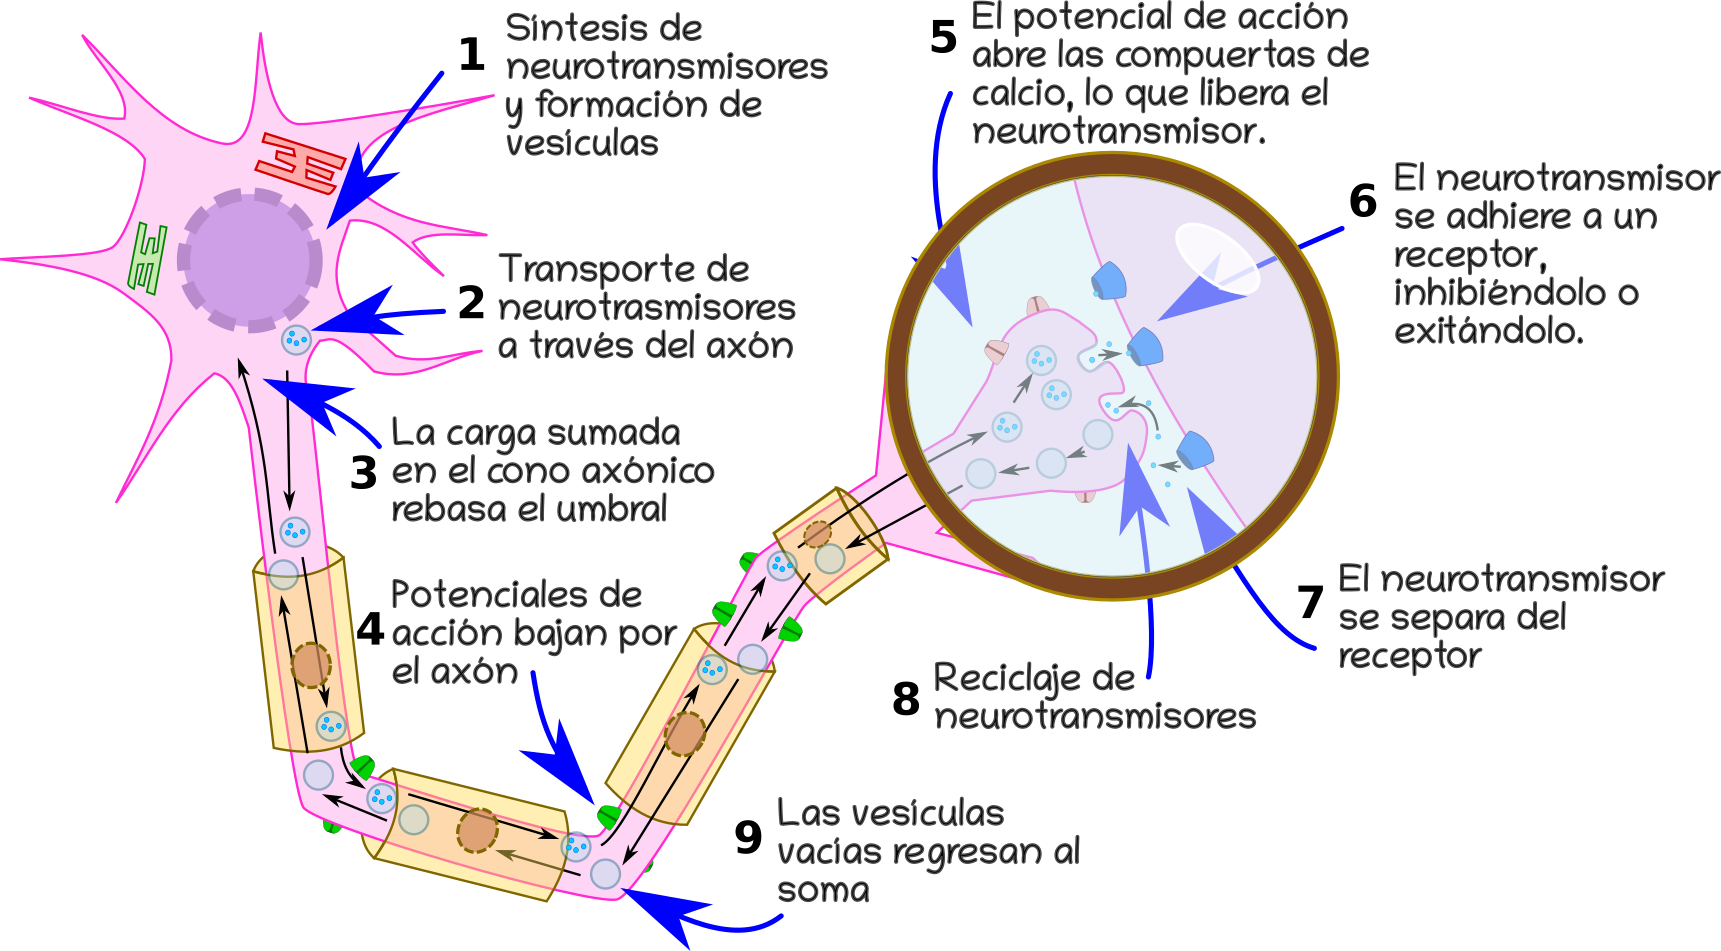
\includegraphics[scale=0.2]{../Figuras/neurotransmision.png} 
 \caption{Esquema detallado de una neurotransmisión. Author: Verónica Arriola Rios.}
 \label{fig:nTransmision}
\end{figure}

La neurona (típica) a lo largo de su axón, está cubierta de nodos (y de células de mielina). Estos nodos están para evitar que se distorsionen o se pierda la señal recibida en la dendritas, en ellos se recarga la señal para que llegue hasta el soma de la neurona. Donde se mandará o no una respuesta, un pulso eléctrico.  


%\begin{figure}[h]
% \centering
% 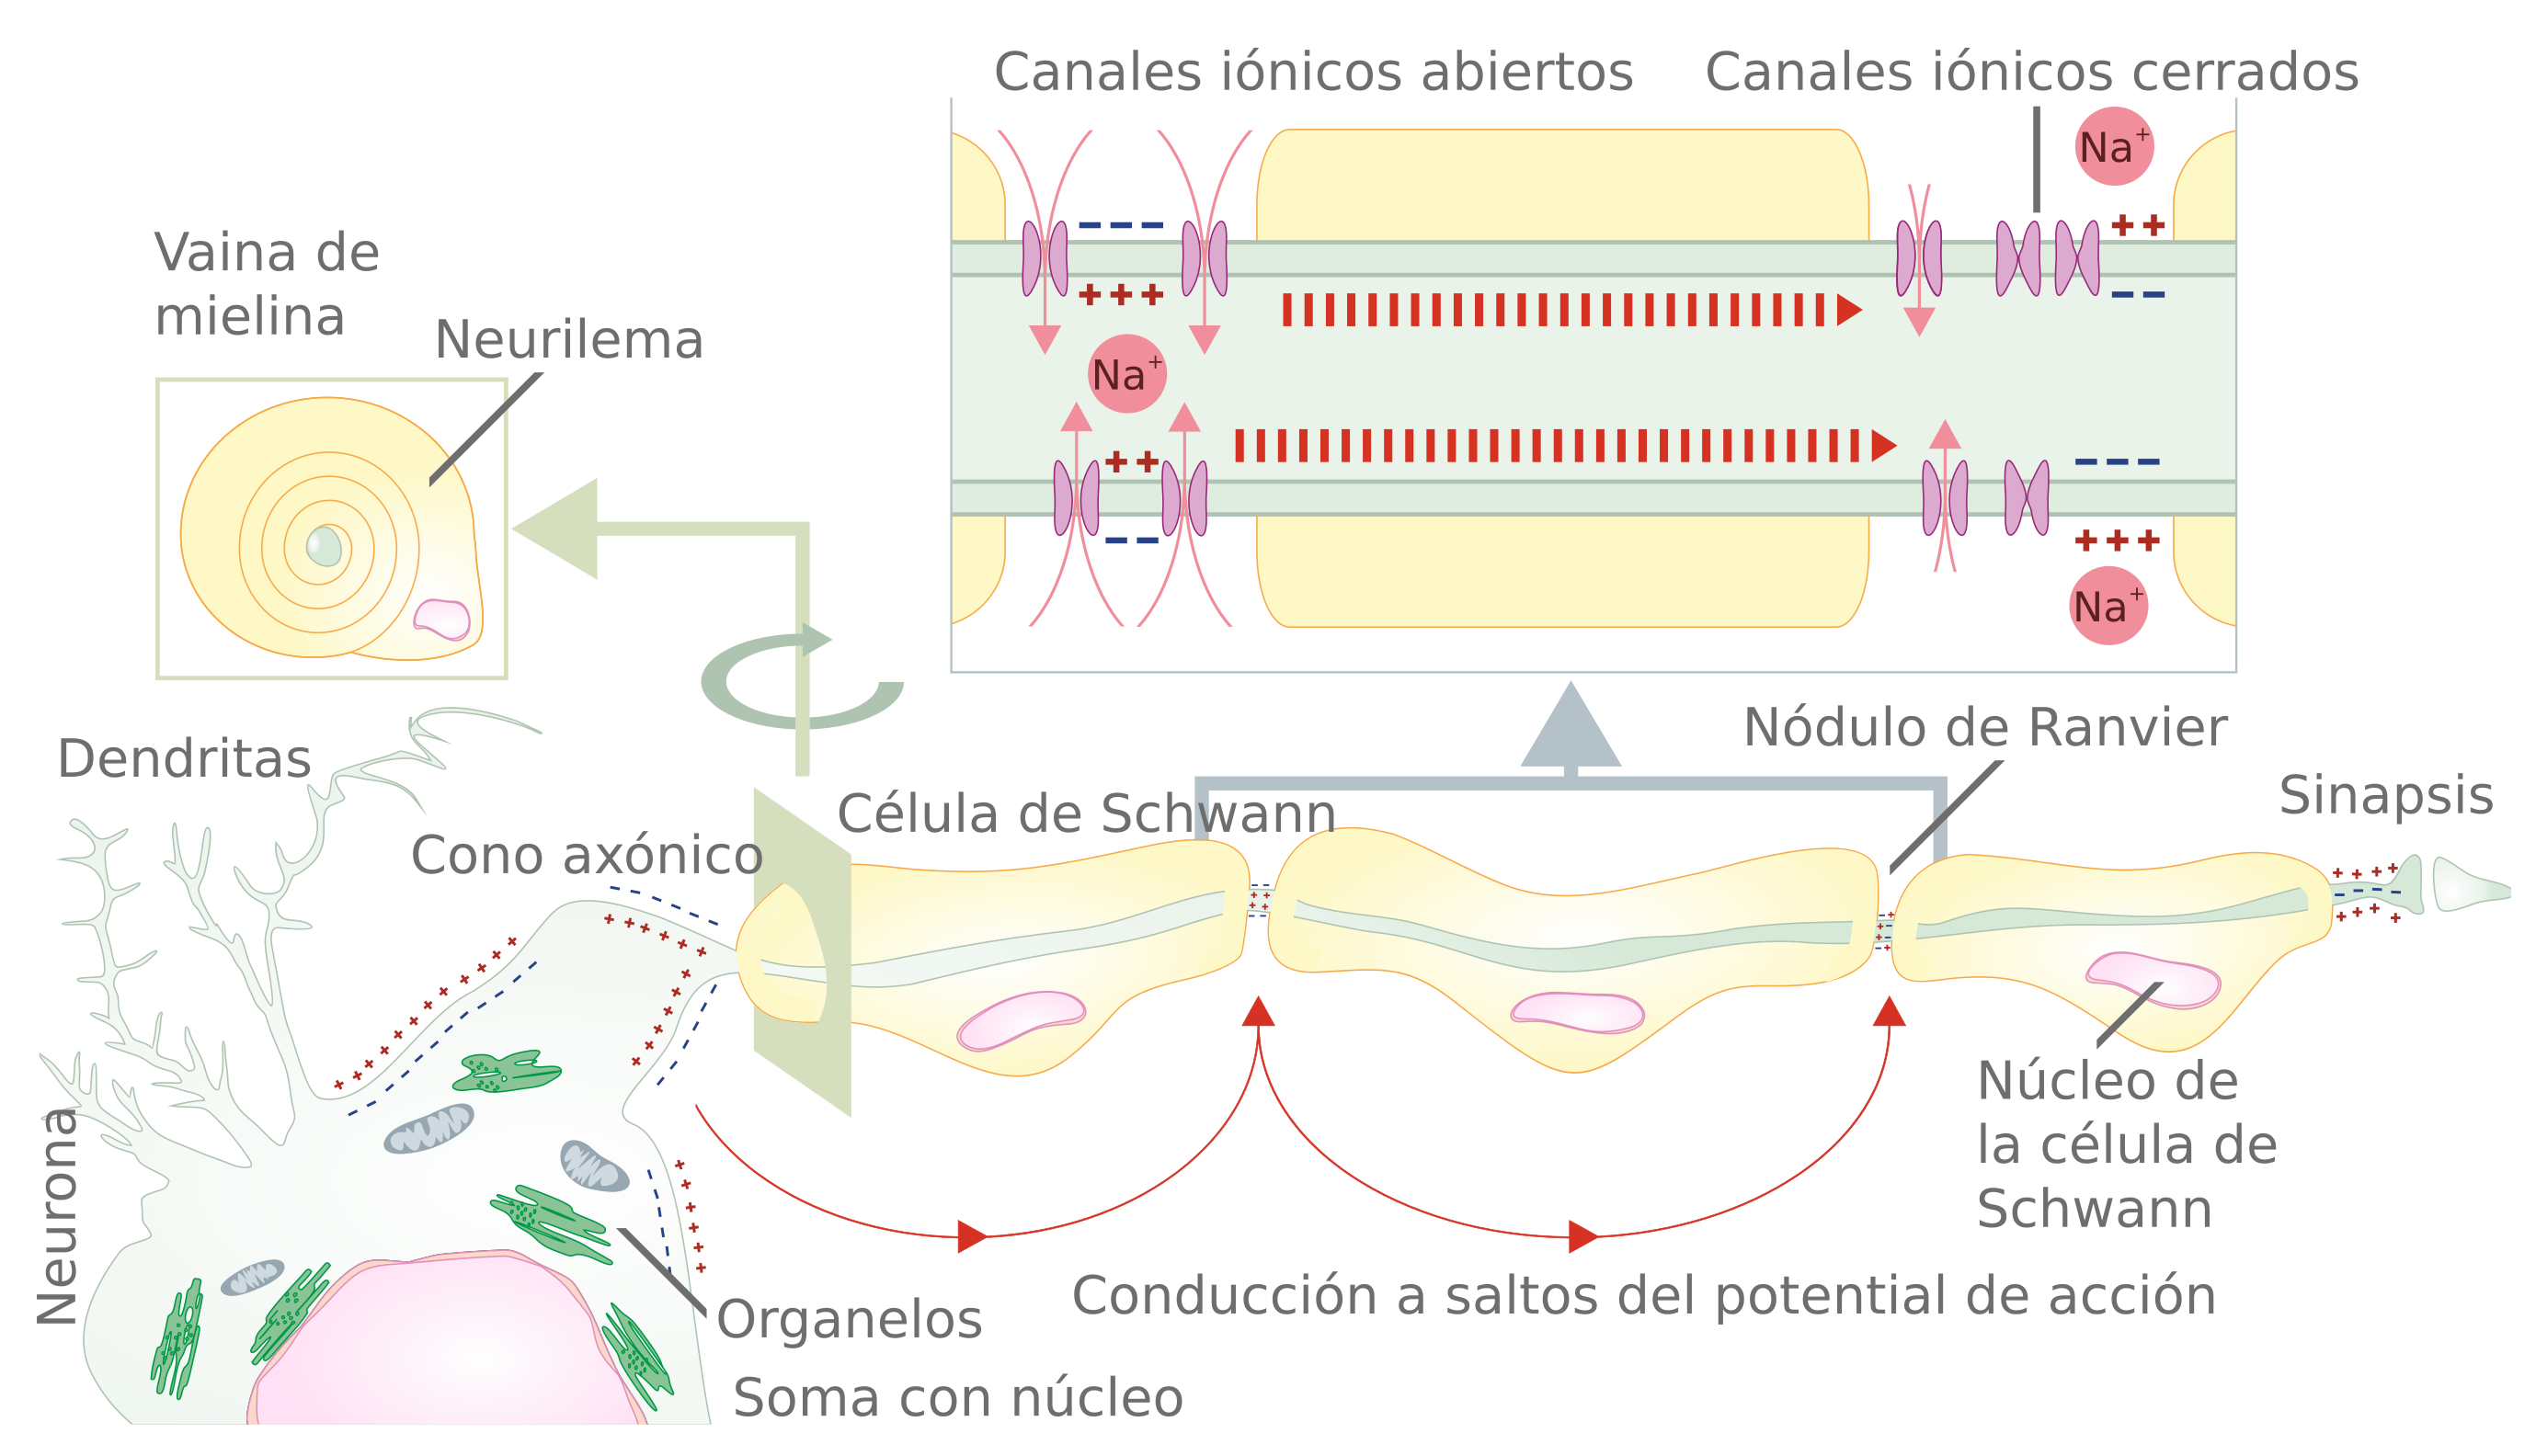
\includegraphics[scale=0.15]{../Figuras/Saltos.png}
% \caption{Corriente iónica por el axón (efecto de corto plazo), Helixitta, 1 octubre 2015, Wikimedia Commons, \url{https://commons.wikimedia.org/wiki/File:Propagation_of_action_potential_along_myelinated_nerve_fiber_en.svg}, Creative Commons Attribution-ShareAlike 4.0 International}
% \label{fig:conduccionSaltos}
%\end{figure}


%Este trayecto puede ir de una neurona a unas pocas neuronas vecinas, hasta unos cuantos metros (ej. esta podría estar en la médula espinal y el axón llegar hasta el dedo del pie). Cuando la señal llega a la terminal del axón, hay varias terminales que van a reaccionar ante el cambio de electricidad mediante la liberación de unas vesículas, que contienen \textbf{neurotransmisores}.


 % Pensemos en la neurona como toda una compuerta, por un lado, está el cuerpo de una neurona típica, por otro lado están las dendritas y axones donde tienen lugar la mayoría de las reacciones que permiten la transmisión de información.  La forma en que fluye esta información es mediante sustancias químicas (neurotransmisores) y iones ($Na+, K+, Cl-$, etc.) que se están intercambiando entre la parte de afuera y de adentro de la neurona, a través de su membrana.
 
 %Particularmente en las dendritas y axones se tienen terminaciones que se pueden conectar con otras neuronas y de esta manera permitir el paso de información. En estos puntos de conexión se indentifica a las neuronas participantes como:
 
%La presencia de estos iones provoca que en el interior de la neurona haya una cierta carga eléctrica, mientras que en el exterior (el líquido de afuera) hay otra carga eléctrica, es decir, hay una \textbf{diferencia de potencial} entre el interior y el exterior de la neurona, por eso se dice que la membrana axónica en sí misma tiene una carga eléctrica. Esta membrana es porosa por tanto intercambia partículas con el exterior, esto va a hacer que su polarización varíe con el tiempo, si en algún momento la diferencia de potencial neta rebasa un cierto umbral la neurona emitirá un pulso que afectará a las neuronas con las que esté conectada.


\subsection{Sinapsis}

 Donde dos neuronas en estrecha proximidad, se transmiten información se llama \textbf{sinapsis}. La sinapsis (típica) se establece entre el axón de una neurona y la dendrita de otra neurona. \parencite{sistemaNervioso}%pag50.



\begin{figure}[h]
 \centering
 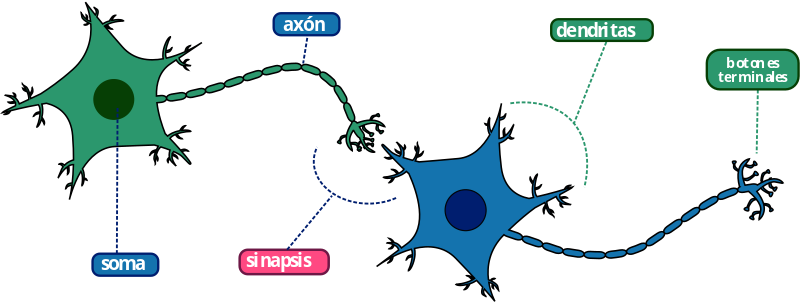
\includegraphics[scale=0.5]{../Figuras/Part_of_neurons_in_Spanish.png}
 \caption{Part of neurons in Spanish, Dana Scarinci Zabaleta, 24 February 2019, Wikimedia Commons, \url{https://commons.wikimedia.org/wiki/File:Part_of_neurons_in_Spanish.svg}, OpenStax, CC0}
 \label{fig:sinapsisN}
\end{figure}


\subsubsection{Clasificación de sinapsis}

Los dos tipos de sinapsis (relevantes para el curso) son:

\begin{description}
 \item [Sinapsis eléctrica:] las membranas de las células pre y post sinápticas se unen en la brecha sináptica, que son pequeños canales que permiten el paso de iones (\fref{fig:sinapsisN}).

	%\begin{enumerate}
  	% \item Posee una transmisión bidireccional de los potenciales de acción.
  	% \item Sincronización en la actividad neuronal, lo cual hace posible una acción coordinada.
 	% \item Los potenciales de acción pasan a través del canal proteico directamente sin necesidad de la liberación de los neurotransmisores, por tanto, es más rápida.
	%\end{enumerate}


\begin{figure}[h]
 \centering
 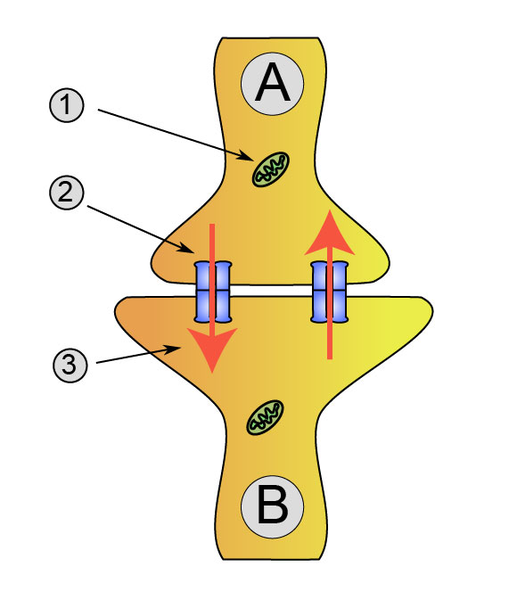
\includegraphics[scale=0.2]{../Figuras/sinapsisElectrica.png}
 \caption{Synaptical transmission (electrical). Neurona A transmisora, Neurona B receptora, 1. Mitocondria, 2. Uniones gap formadas por conexiones, 3. Señal eléctrica, Nrets~commonswiki, 23 September 2005, Wikimedia Commons, \url{https://commons.wikimedia.org/wiki/File:Synapse_diag2.png}, Inkscape 0.42, CC-BY-SA 3.0}
 \label{fig:sinapsisN}
\end{figure}
 
 \item [Sinapsis química:] la neurona libera moléculas neurotransmisoras a otra neurona adyacente en un pequeño espacio, la brecha sináptica (\fref{fig:sinapsisQ}). %Sus cuatro etapas principales son:

%\begin{enumerate}
% \item Un potencial de acción llega al botón terminal proveniente desde el cono axónico.
% \item Los neurotransmisores contenidos en las vesículas que están él los botones terminales, son liberados en la brecha sináptica y se dispersan.
% \item Cada neurotransmisor se une a su receptor ubicado en la membrana de la neurona postsináptica.
% \item El exceso de neurotransmisores que queda en el espacio sináptico es degradado o recaptado.
%\end{enumerate}


\begin{figure}[h]
 \centering
 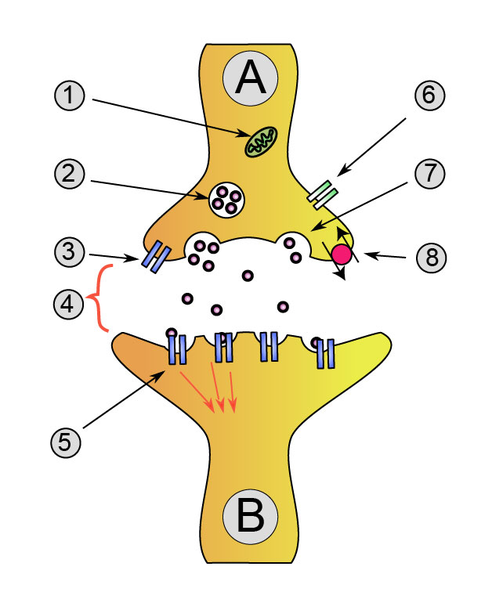
\includegraphics[scale=0.2]{../Figuras/SinapsisQuimica1.png}
 \caption{Synaptical transmission (chemical). Neurona A transmisora, Neurona B receptora, 1. Mitocondria, 2. Vesícula sináptica llena de neurotransmisor, 3. Autorreceptor, 4. Brecha sináptica, 5. Receptor de neurotransmisores, 6. Canal de calcio, 7. Neurotransmisor liberador de vesículas fusionadas, 8. Bomba de recaptación de neurotransmisores, Utilisateur:Dake, 23 September 2005, Wikimedia Commons, \url{https://commons.wikimedia.org/wiki/File:Synapse_diag1.png}, Inkscape 0.42, CC-BY-SA 3.0}
 \label{fig:sinapsisQ}
\end{figure}

\end{description}








\subsection{Señal eléctrica}

El paso de las señales eléctricas entre neuronas, se dan gracias a los canales de iones, los que destacan son los siguientes:

\begin{itemize}
\item \textbf{Canal por fuga:} Estos se abren y cierran aleatoriamente, todo el tiempo están activos en la neurona. Por ejemplo: sodio y potasio.

\item \textbf{Canal regulado por ligado:} En este un neurotransmisor que es el que provocar o impide que se abran. 

\item  \textbf{Canal por estímulo mecánico:} Permiten que pasen más iones o menos iones dependiendo, si se ejerció una presión, por ejemplo, con las neuronas cerca de la piel.
\item \textbf{Canales regulados por el voltaje:} Un voltaje, es el que abre o cierra el canal. Permite o no el paso del pulso eléctrico. % Existen una variante de este tipo, el cual tiene una pequeña compuerta abajo, que la puede cerrar independientemente.
\end{itemize}


Existen realmente una buena cantidad de iones presentes en el cerebro, pero los más protagónicos son \textbf{potasio}, el \textbf{sodio} y el \textbf{cloro}. Los que vamos a utilizar para un modelo matemático de las neuronas. 


\begin{figure}[h]
 \centering
 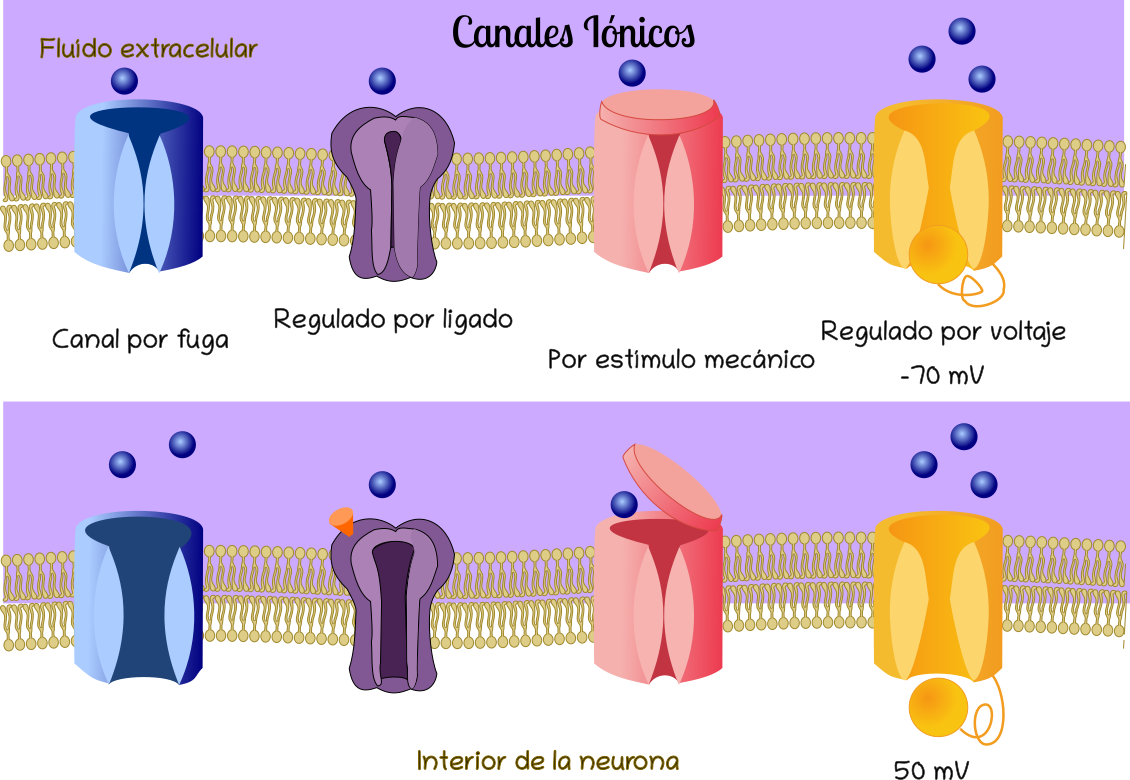
\includegraphics[scale=0.28]{../Figuras/canalesIonicos.png}
 \caption{Representación de la clasificación de los canales iónicos.}
 \label{fig:MembranaP}
\end{figure}



\subsubsection{Neuroplasticidad}

Una característica importante de la conexión entre neuronas es la neuroplasticidad, que es lo que nos permite el aprendizaje a largo plazo en el cerebro, es un mecanismo de aprendizaje del cerebro en el cual cuando las neuronas se activan simultáneamente con frecuencia la conexión entre ellas se fortalece.


Este mecanismo constituye la principal inspiración para el diseño de las redes neuronales artificiales, concretamente en esto se inspiran los algoritmos de entrenamiento. Calculamos, qué conexiones debemos reforzar y cuáles debemos de debilitar para que nuestras redes neuronales calculen las funciones que a nosotros nos interesan.


Comentario Importante a preguntar:
En esta sección estaba también explicado el paso de iones por la membrana, pero no sé si sea relevante en esta sección o mejor directamente en el modelo de HH, que es lo importante para sus prácticas de lab.

\begin{figure}[h]
 \centering
 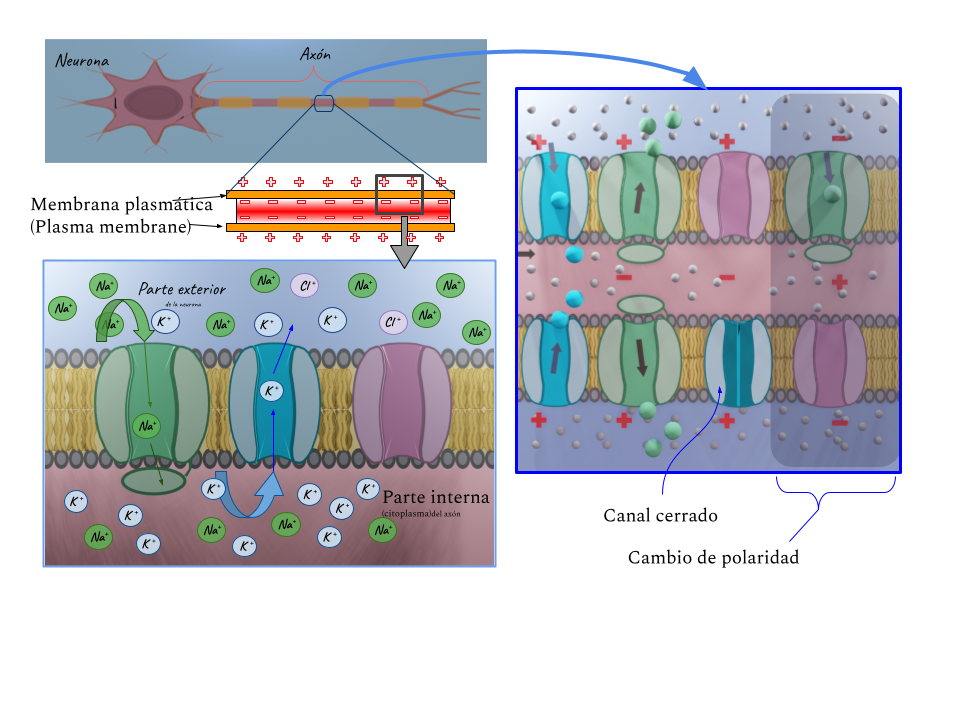
\includegraphics[scale=0.5]{../Figuras/MembranaP.png}
 \caption{Representación de la membrana axónica en potencial de reposo en la parte inferior izquierda, y en la parte derecha con un estímulo que genera el cambio de polaridad en la misma, así como el cierre de canales y paso de iones.}
 \label{fig:MembranaP}
\end{figure}


%En breve \textbf{¿Qué son las neuronas?} 
%La neurona es un tipo de célula perteneciente al sistema nervioso central, que se comunica tanto por señales eléctricas como por señales químicas. Son células con núcleo, sus cuerpos tienen uno o varios axones y dendritas con la habilidad de transferir electricidad. Permite transmitir un pulso eléctrico desde el soma (a través sus membranas) pasando por los nodos, hasta las dendritas. Para soltar el pulso eléctrico, en espera que otras (dendritas) neuronas recuperen el pulso eléctrico.\parencite{neurona_A_cerebro}







